\newpage
\texHeader
\hypertarget{projectStructure tex}{}
\subsection{Your MOSL workspace}

As you now know, eMoflon is a plug-in for Eclipse. More precisely, eMoflon requires the Eclipse Modeling Framework (EMF) in order to work. EMF uses two separate
models, a Genmodel and an Ecore model, for code generation. The Genmodel contains boring information about code generation such as path, file prefixes, and
other information. We are more interested in the Ecore model, which we specify with MOSL.

When you switched the ``Top Level Elements'' from \texttt{Projects} to \texttt{Working Sets}, you noticed that a few extra nodes were displayed in the project
browser. Each node you see has different criteria for grouping related Eclipse Projects together, which makes them your project \emph{working sets}.

The \texttt{Specifications} working set contains all \emph{metamodel projects} in a workspace (Fig.~\ref{fig_modelSpecification}). This means that for every
new metamodel you create in your current workspace, all of the relevant files will be placed here.

 \begin{figure}[htbp]
  \centering
  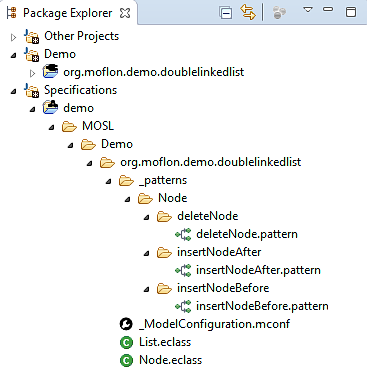
\includegraphics[width=0.6\textwidth]{eclipse_Specification}
  \caption{Specification working set}
  \label{fig_modelSpecification}
\end{figure}
  
Let's have a look at the two \emph{eclass} files. While you can combine several short class declarations in a single file in some languages (such as Java),
each class is kept separated in its own file when using MOSL.

Inspect the file \texttt{List.eclass}, and you'll see it has a just one \emph{EAttribute}. EAttributes are defined by their name, followed by a colon
symbol and type. This class also has one \emph{EReference}, a \emph{container reference}. This is represented by the diamond operator in front of an arrow.
Switch to the \texttt{Node} eclass and you can observe the second reference type, a \emph{simple~reference}. It's represented by a plain arrow. EReference names are
immediately followed by their multiplicity and then, similar to an attribute, a colon and their type of the referenced EClass (i.e., the target of the arrow).

In the \texttt{Node} eclass (Fig.~\ref{fig_patternDeleteNode}), a few methods have been declared. You can see that each function is remarkably small. In fact,
the only thing the functions are doing are invoking \emph{patterns}. These patterns represent structural changes, and their container functions are used
exclusively for control flow (i.e., sequences, branches, and loops).

 \begin{figure}[htbp]
  \centering
  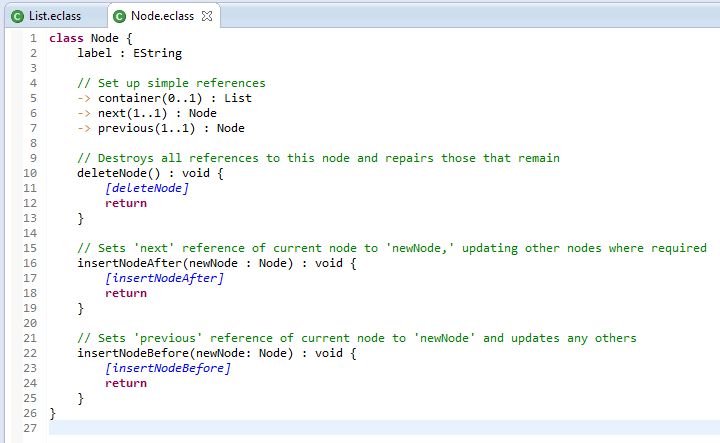
\includegraphics[width=1.0\textwidth]{eclipse_commentsNode}
  \caption{The \texttt{Node} eclass}
  \label{fig_eclassNode}
\end{figure}

% See how it looks.. may have to remove
%\nxtPage{\thepage}

After many long discussions, it was decided that patterns should always be implemented in separate files. Inspect Fig.~\ref{fig_modelSpecification} again, and
observe the locations where the patterns are placed. You'll notice that there is a folder for the \texttt{Node} eclass, and a subfolder for each method. There's
no folder for \texttt{List} because it never calls a pattern.

Check out the \texttt{deleteNode} pattern (Fig ~\ref{fig_patternDeleteNode}).

 \begin{figure}[htbp]
  \centering
  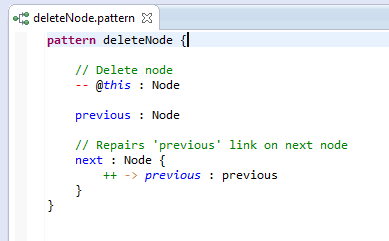
\includegraphics[width=0.6\textwidth]{eclipse_patternDeleteNode}
  \caption{Eclipse: The deleteNode Pattern}
  \label{fig_patternDeleteNode}
\end{figure}

You can see that there is a destroy command on \texttt{@this}, denoted by ``--''. It gets rid of the node, but it doesn't do anything about the previous and
next references defined on it (remember that we're dealing with a double linked list here!). That's because when the node is removed, everything attached to it
will be automatically cleaned and updated. The final command reconnects the next and previous nodes of the deleted node to close the 'hole' in the list. this is
accomplished by setting (``++'') the previous reference of the next node to the previous node.
 
So that's a quick overview of the MOSL language but, how do we generate code from all of this?

%\fancyfoot[R]{  $\triangleright$ \hyperlink{codeGen common}{Next} }

First, eMoflon does not generate code with every change. To improve performance, only the parser is invoked when you save files. This means
that to generate code for the project, you need to either invoke the \texttt{Build (and clean)} command from the eMoflon context menu after right clicking your
metamodel project, or by navigating to the ``Build (without cleaning)'' button next to the ``New Metamodel'' button. Cleaning means\ldots
